\documentclass[1p]{elsarticle_modified}
%\bibliographystyle{elsarticle-num}

%\usepackage[colorlinks]{hyperref}
%\usepackage{abbrmath_seonhwa} %\Abb, \Ascr, \Acal ,\Abf, \Afrak
\usepackage{amsfonts}
\usepackage{amssymb}
\usepackage{amsmath}
\usepackage{amsthm}
\usepackage{scalefnt}
\usepackage{amsbsy}
\usepackage{kotex}
\usepackage{caption}
\usepackage{subfig}
\usepackage{color}
\usepackage{graphicx}
\usepackage{xcolor} %% white, black, red, green, blue, cyan, magenta, yellow
\usepackage{float}
\usepackage{setspace}
\usepackage{hyperref}

\usepackage{tikz}
\usetikzlibrary{arrows}

\usepackage{multirow}
\usepackage{array} % fixed length table
\usepackage{hhline}

%%%%%%%%%%%%%%%%%%%%%
\makeatletter
\renewcommand*\env@matrix[1][\arraystretch]{%
	\edef\arraystretch{#1}%
	\hskip -\arraycolsep
	\let\@ifnextchar\new@ifnextchar
	\array{*\c@MaxMatrixCols c}}
\makeatother %https://tex.stackexchange.com/questions/14071/how-can-i-increase-the-line-spacing-in-a-matrix
%%%%%%%%%%%%%%%

\usepackage[normalem]{ulem}

\newcommand{\msout}[1]{\ifmmode\text{\sout{\ensuremath{#1}}}\else\sout{#1}\fi}
%SOURCE: \msout is \stkout macro in https://tex.stackexchange.com/questions/20609/strikeout-in-math-mode

\newcommand{\cancel}[1]{
	\ifmmode
	{\color{red}\msout{#1}}
	\else
	{\color{red}\sout{#1}}
	\fi
}

\newcommand{\add}[1]{
	{\color{blue}\uwave{#1}}
}

\newcommand{\replace}[2]{
	\ifmmode
	{\color{red}\msout{#1}}{\color{blue}\uwave{#2}}
	\else
	{\color{red}\sout{#1}}{\color{blue}\uwave{#2}}
	\fi
}

\newcommand{\Sol}{\mathcal{S}} %segment
\newcommand{\D}{D} %diagram
\newcommand{\A}{\mathcal{A}} %arc


%%%%%%%%%%%%%%%%%%%%%%%%%%%%%5 test

\def\sl{\operatorname{\textup{SL}}(2,\Cbb)}
\def\psl{\operatorname{\textup{PSL}}(2,\Cbb)}
\def\quan{\mkern 1mu \triangleright \mkern 1mu}

\theoremstyle{definition}
\newtheorem{thm}{Theorem}[section]
\newtheorem{prop}[thm]{Proposition}
\newtheorem{lem}[thm]{Lemma}
\newtheorem{ques}[thm]{Question}
\newtheorem{cor}[thm]{Corollary}
\newtheorem{defn}[thm]{Definition}
\newtheorem{exam}[thm]{Example}
\newtheorem{rmk}[thm]{Remark}
\newtheorem{alg}[thm]{Algorithm}

\newcommand{\I}{\sqrt{-1}}
\begin{document}

%\begin{frontmatter}
%
%\title{Boundary parabolic representations of knots up to 8 crossings}
%
%%% Group authors per affiliation:
%\author{Yunhi Cho} 
%\address{Department of Mathematics, University of Seoul, Seoul, Korea}
%\ead{yhcho@uos.ac.kr}
%
%
%\author{Seonhwa Kim} %\fnref{s_kim}}
%\address{Center for Geometry and Physics, Institute for Basic Science, Pohang, 37673, Korea}
%\ead{ryeona17@ibs.re.kr}
%
%\author{Hyuk Kim}
%\address{Department of Mathematical Sciences, Seoul National University, Seoul 08826, Korea}
%\ead{hyukkim@snu.ac.kr}
%
%\author{Seokbeom Yoon}
%\address{Department of Mathematical Sciences, Seoul National University, Seoul, 08826,  Korea}
%\ead{sbyoon15@snu.ac.kr}
%
%\begin{abstract}
%We find all boundary parabolic representation of knots up to 8 crossings.
%
%\end{abstract}
%\begin{keyword}
%    \MSC[2010] 57M25 
%\end{keyword}
%
%\end{frontmatter}

%\linenumbers
%\tableofcontents
%
\newcommand\colored[1]{\textcolor{white}{\rule[-0.35ex]{0.8em}{1.4ex}}\kern-0.8em\color{red} #1}%
%\newcommand\colored[1]{\textcolor{white}{ #1}\kern-2.17ex	\textcolor{white}{ #1}\kern-1.81ex	\textcolor{white}{ #1}\kern-2.15ex\color{red}#1	}

{\Large $\underline{12a_{0112}~(K12a_{0112})}$}

\setlength{\tabcolsep}{10pt}
\renewcommand{\arraystretch}{1.6}
\vspace{1cm}\begin{tabular}{m{100pt}>{\centering\arraybackslash}m{274pt}}
\multirow{5}{120pt}{
	\centering
	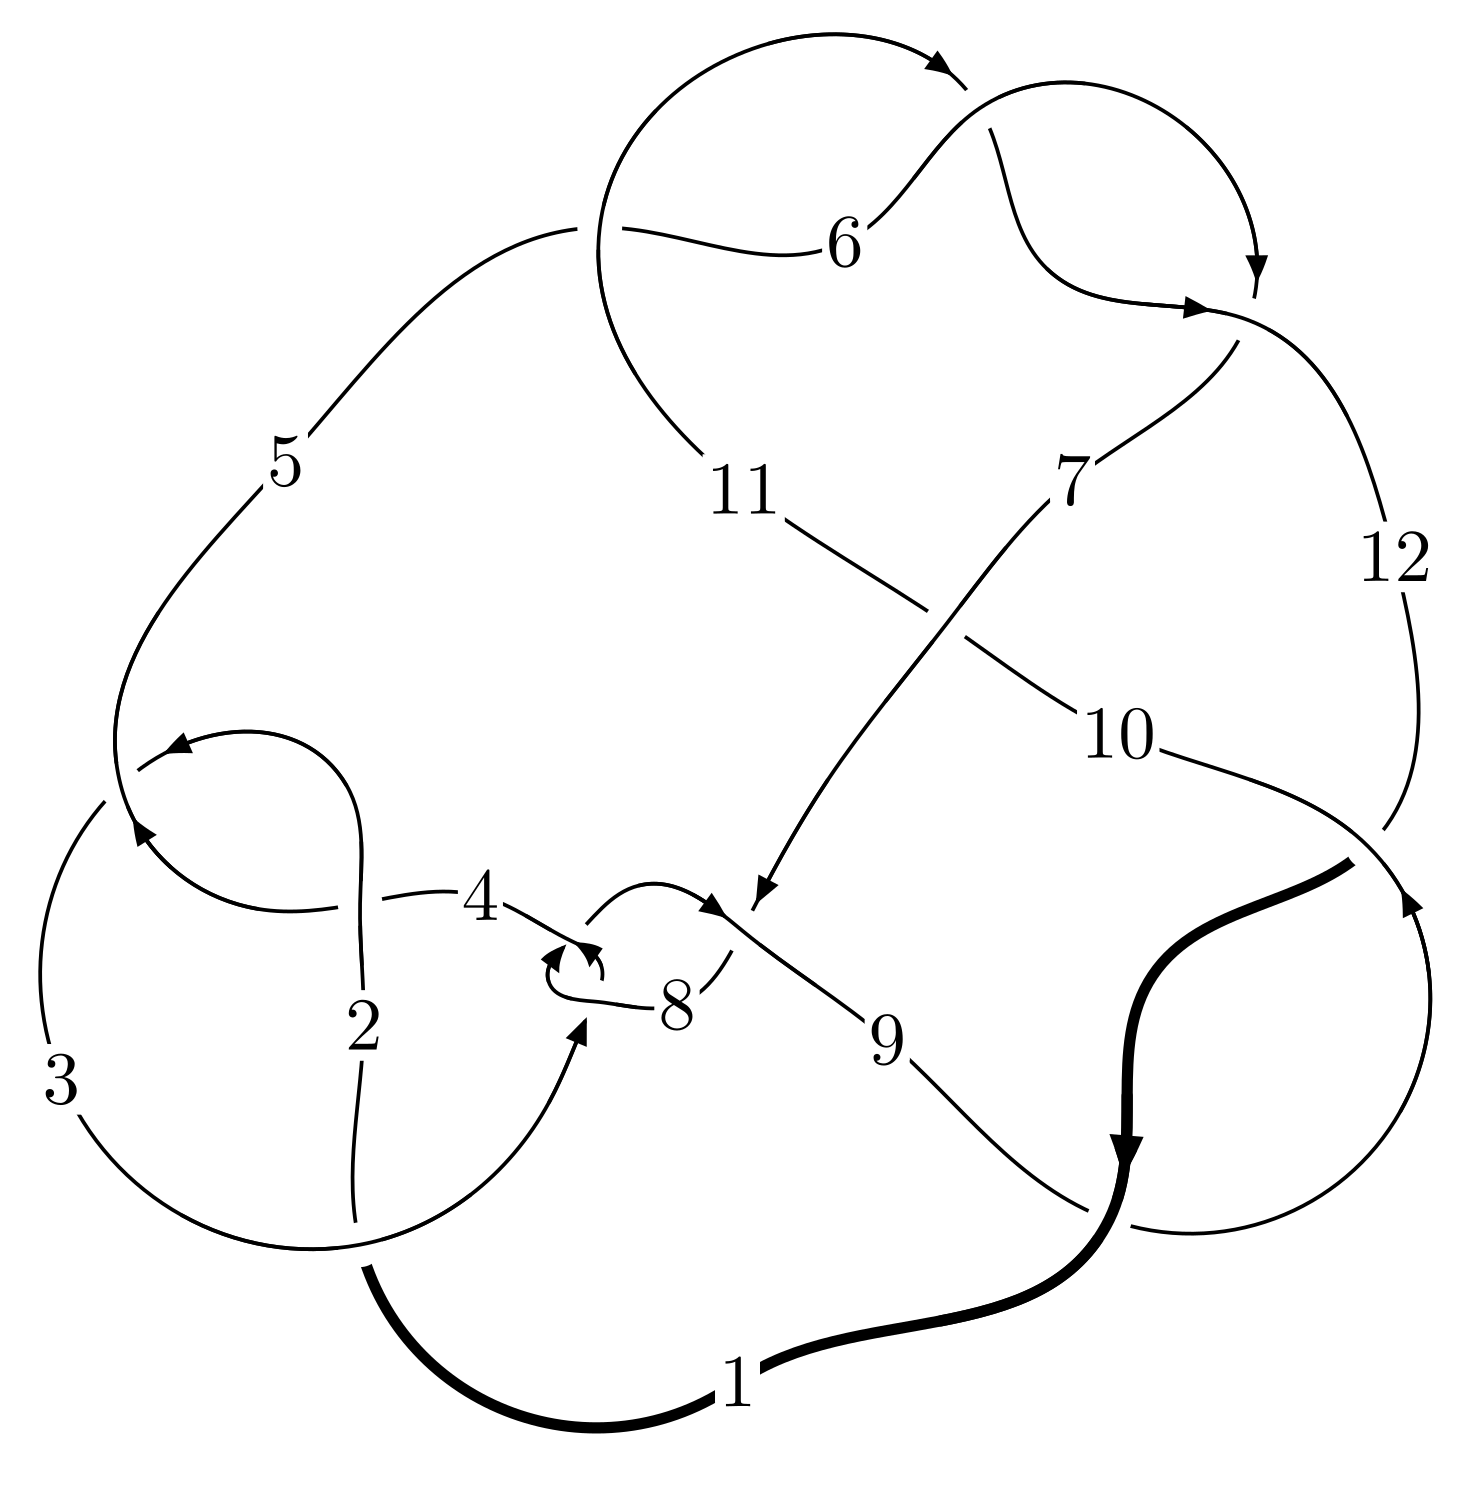
\includegraphics[width=112pt]{../../../GIT/diagram.site/Diagrams/png/913_12a_0112.png}\\
\ \ \ A knot diagram\footnotemark}&
\allowdisplaybreaks
\textbf{Linearized knot diagam} \\
\cline{2-2}
 &
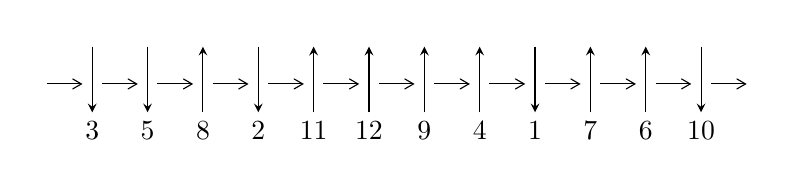
\begin{tikzpicture}[x=20pt, y=17pt]
	% nodes
	\node (C0) at (0, 0) {};
	\node (C1) at (1, 0) {};
	\node (C1U) at (1, +1) {};
	\node (C1D) at (1, -1) {3};

	\node (C2) at (2, 0) {};
	\node (C2U) at (2, +1) {};
	\node (C2D) at (2, -1) {5};

	\node (C3) at (3, 0) {};
	\node (C3U) at (3, +1) {};
	\node (C3D) at (3, -1) {8};

	\node (C4) at (4, 0) {};
	\node (C4U) at (4, +1) {};
	\node (C4D) at (4, -1) {2};

	\node (C5) at (5, 0) {};
	\node (C5U) at (5, +1) {};
	\node (C5D) at (5, -1) {11};

	\node (C6) at (6, 0) {};
	\node (C6U) at (6, +1) {};
	\node (C6D) at (6, -1) {12};

	\node (C7) at (7, 0) {};
	\node (C7U) at (7, +1) {};
	\node (C7D) at (7, -1) {9};

	\node (C8) at (8, 0) {};
	\node (C8U) at (8, +1) {};
	\node (C8D) at (8, -1) {4};

	\node (C9) at (9, 0) {};
	\node (C9U) at (9, +1) {};
	\node (C9D) at (9, -1) {1};

	\node (C10) at (10, 0) {};
	\node (C10U) at (10, +1) {};
	\node (C10D) at (10, -1) {7};

	\node (C11) at (11, 0) {};
	\node (C11U) at (11, +1) {};
	\node (C11D) at (11, -1) {6};

	\node (C12) at (12, 0) {};
	\node (C12U) at (12, +1) {};
	\node (C12D) at (12, -1) {10};
	\node (C13) at (13, 0) {};

	% arrows
	\draw[->,>={angle 60}]
	(C0) edge (C1) (C1) edge (C2) (C2) edge (C3) (C3) edge (C4) (C4) edge (C5) (C5) edge (C6) (C6) edge (C7) (C7) edge (C8) (C8) edge (C9) (C9) edge (C10) (C10) edge (C11) (C11) edge (C12) (C12) edge (C13) ;	\draw[->,>=stealth]
	(C1U) edge (C1D) (C2U) edge (C2D) (C3D) edge (C3U) (C4U) edge (C4D) (C5D) edge (C5U) (C6D) edge (C6U) (C7D) edge (C7U) (C8D) edge (C8U) (C9U) edge (C9D) (C10D) edge (C10U) (C11D) edge (C11U) (C12U) edge (C12D) ;
	\end{tikzpicture} \\
\hhline{~~} \\& 
\textbf{Solving Sequence} \\ \cline{2-2} 
 &
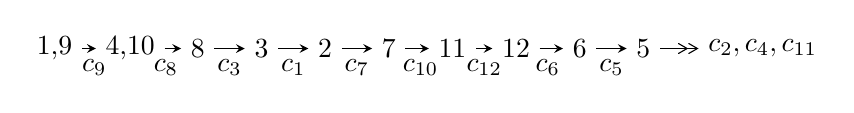
\begin{tikzpicture}[x=23pt, y=7pt]
	% node
	\node (A0) at (-1/8, 0) {1,9};
	\node (A1) at (17/16, 0) {4,10};
	\node (A2) at (17/8, 0) {8};
	\node (A3) at (25/8, 0) {3};
	\node (A4) at (33/8, 0) {2};
	\node (A5) at (41/8, 0) {7};
	\node (A6) at (49/8, 0) {11};
	\node (A7) at (57/8, 0) {12};
	\node (A8) at (65/8, 0) {6};
	\node (A9) at (73/8, 0) {5};
	\node (C1) at (1/2, -1) {$c_{9}$};
	\node (C2) at (13/8, -1) {$c_{8}$};
	\node (C3) at (21/8, -1) {$c_{3}$};
	\node (C4) at (29/8, -1) {$c_{1}$};
	\node (C5) at (37/8, -1) {$c_{7}$};
	\node (C6) at (45/8, -1) {$c_{10}$};
	\node (C7) at (53/8, -1) {$c_{12}$};
	\node (C8) at (61/8, -1) {$c_{6}$};
	\node (C9) at (69/8, -1) {$c_{5}$};
	\node (A10) at (11, 0) {$c_{2},c_{4},c_{11}$};

	% edge
	\draw[->,>=stealth]	
	(A0) edge (A1) (A1) edge (A2) (A2) edge (A3) (A3) edge (A4) (A4) edge (A5) (A5) edge (A6) (A6) edge (A7) (A7) edge (A8) (A8) edge (A9) ;
	\draw[->>,>={angle 60}]	
	(A9) edge (A10);
\end{tikzpicture} \\ 

\end{tabular} \\

\footnotetext{
The image of knot diagram is generated by the software ``\textbf{Draw programme}" developed by Andrew Bartholomew(\url{http://www.layer8.co.uk/maths/draw/index.htm\#Running-draw}), where we modified some parts for our purpose(\url{https://github.com/CATsTAILs/LinksPainter}).
}\phantom \\ \newline 
\centering \textbf{Ideals for irreducible components\footnotemark of $X_{\text{par}}$} 
 
\begin{align*}
I^u_{1}&=\langle 
6.90259\times10^{236} u^{87}+8.88875\times10^{237} u^{86}+\cdots+2.40669\times10^{238} b-4.89965\times10^{238},\\
\phantom{I^u_{1}}&\phantom{= \langle  }6.80069\times10^{238} u^{87}+9.46673\times10^{239} u^{86}+\cdots+5.53539\times10^{239} a+2.08834\times10^{241},\\
\phantom{I^u_{1}}&\phantom{= \langle  }u^{88}+14 u^{87}+\cdots+3387 u+207\rangle \\
I^u_{2}&=\langle 
b,\;- u^4- u^3-2 u^2+a- u-1,\;u^5+u^4+2 u^3+u^2+u+1\rangle \\
\\
\end{align*}
\raggedright * 2 irreducible components of $\dim_{\mathbb{C}}=0$, with total 93 representations.\\
\footnotetext{All coefficients of polynomials are rational numbers. But the coefficients are sometimes approximated in decimal forms when there is not enough margin.}
\newpage
\renewcommand{\arraystretch}{1}
\centering \section*{I. $I^u_{1}= \langle 6.90\times10^{236} u^{87}+8.89\times10^{237} u^{86}+\cdots+2.41\times10^{238} b-4.90\times10^{238},\;6.80\times10^{238} u^{87}+9.47\times10^{239} u^{86}+\cdots+5.54\times10^{239} a+2.09\times10^{241},\;u^{88}+14 u^{87}+\cdots+3387 u+207 \rangle$}
\flushleft \textbf{(i) Arc colorings}\\
\begin{tabular}{m{7pt} m{180pt} m{7pt} m{180pt} }
\flushright $a_{1}=$&$\begin{pmatrix}0\\u\end{pmatrix}$ \\
\flushright $a_{9}=$&$\begin{pmatrix}1\\0\end{pmatrix}$ \\
\flushright $a_{4}=$&$\begin{pmatrix}-0.122858 u^{87}-1.71022 u^{86}+\cdots-627.195 u-37.7271\\-0.0286808 u^{87}-0.369335 u^{86}+\cdots+21.4446 u+2.03584\end{pmatrix}$ \\
\flushright $a_{10}=$&$\begin{pmatrix}1\\u^2\end{pmatrix}$ \\
\flushright $a_{8}=$&$\begin{pmatrix}-0.00171350 u^{87}-0.0279250 u^{86}+\cdots-36.0867 u-5.51864\\-0.0374023 u^{87}-0.488646 u^{86}+\cdots-233.414 u-15.5951\end{pmatrix}$ \\
\flushright $a_{3}=$&$\begin{pmatrix}-0.0424549 u^{87}-0.597700 u^{86}+\cdots-379.570 u-27.2479\\-0.0311366 u^{87}-0.382954 u^{86}+\cdots+100.315 u+8.26440\end{pmatrix}$ \\
\flushright $a_{2}=$&$\begin{pmatrix}0.0694474 u^{87}+0.975047 u^{86}+\cdots+215.246 u+12.4910\\0.0385643 u^{87}+0.496854 u^{86}+\cdots+44.9227 u+3.00962\end{pmatrix}$ \\
\flushright $a_{7}=$&$\begin{pmatrix}0.0356888 u^{87}+0.460721 u^{86}+\cdots+197.327 u+10.0764\\-0.0374023 u^{87}-0.488646 u^{86}+\cdots-233.414 u-15.5951\end{pmatrix}$ \\
\flushright $a_{11}=$&$\begin{pmatrix}0.0269231 u^{87}+0.335328 u^{86}+\cdots+210.971 u+21.3838\\-0.0159512 u^{87}-0.217071 u^{86}+\cdots+26.5351 u+1.10107\end{pmatrix}$ \\
\flushright $a_{12}=$&$\begin{pmatrix}u\\u^3+u\end{pmatrix}$ \\
\flushright $a_{6}=$&$\begin{pmatrix}0.0237817 u^{87}+0.326428 u^{86}+\cdots+315.117 u+18.5023\\-0.0404086 u^{87}-0.542338 u^{86}+\cdots-222.919 u-13.8773\end{pmatrix}$ \\
\flushright $a_{5}=$&$\begin{pmatrix}-0.0753384 u^{87}-1.01734 u^{86}+\cdots-399.712 u-21.7576\\0.00393597 u^{87}+0.0453448 u^{86}+\cdots-0.284989 u-0.354695\end{pmatrix}$\\&\end{tabular}
\flushleft \textbf{(ii) Obstruction class $= -1$}\\~\\
\flushleft \textbf{(iii) Cusp Shapes $= -0.114811 u^{87}-1.49279 u^{86}+\cdots-618.725 u-34.0945$}\\~\\
\newpage\renewcommand{\arraystretch}{1}
\flushleft \textbf{(iv) u-Polynomials at the component}\newline \\
\begin{tabular}{m{50pt}|m{274pt}}
Crossings & \hspace{64pt}u-Polynomials at each crossing \\
\hline $$\begin{aligned}c_{1}\end{aligned}$$&$\begin{aligned}
&u^{88}+46 u^{87}+\cdots+7 u+1
\end{aligned}$\\
\hline $$\begin{aligned}c_{2},c_{4}\end{aligned}$$&$\begin{aligned}
&u^{88}-6 u^{87}+\cdots+7 u-1
\end{aligned}$\\
\hline $$\begin{aligned}c_{3},c_{8}\end{aligned}$$&$\begin{aligned}
&u^{88}+u^{87}+\cdots-32 u+32
\end{aligned}$\\
\hline $$\begin{aligned}c_{5},c_{6},c_{11}\end{aligned}$$&$\begin{aligned}
&u^{88}-2 u^{87}+\cdots+u-1
\end{aligned}$\\
\hline $$\begin{aligned}c_{7}\end{aligned}$$&$\begin{aligned}
&u^{88}-33 u^{87}+\cdots-18944 u+1024
\end{aligned}$\\
\hline $$\begin{aligned}c_{9},c_{12}\end{aligned}$$&$\begin{aligned}
&u^{88}-14 u^{87}+\cdots-3387 u+207
\end{aligned}$\\
\hline $$\begin{aligned}c_{10}\end{aligned}$$&$\begin{aligned}
&u^{88}+6 u^{87}+\cdots-4287 u-1585
\end{aligned}$\\
\hline
\end{tabular}\\~\\
\newpage\renewcommand{\arraystretch}{1}
\flushleft \textbf{(v) Riley Polynomials at the component}\newline \\
\begin{tabular}{m{50pt}|m{274pt}}
Crossings & \hspace{64pt}Riley Polynomials at each crossing \\
\hline $$\begin{aligned}c_{1}\end{aligned}$$&$\begin{aligned}
&y^{88}-2 y^{87}+\cdots+17 y+1
\end{aligned}$\\
\hline $$\begin{aligned}c_{2},c_{4}\end{aligned}$$&$\begin{aligned}
&y^{88}-46 y^{87}+\cdots-7 y+1
\end{aligned}$\\
\hline $$\begin{aligned}c_{3},c_{8}\end{aligned}$$&$\begin{aligned}
&y^{88}-33 y^{87}+\cdots-18944 y+1024
\end{aligned}$\\
\hline $$\begin{aligned}c_{5},c_{6},c_{11}\end{aligned}$$&$\begin{aligned}
&y^{88}-82 y^{87}+\cdots+11 y+1
\end{aligned}$\\
\hline $$\begin{aligned}c_{7}\end{aligned}$$&$\begin{aligned}
&y^{88}+35 y^{87}+\cdots+3538944 y+1048576
\end{aligned}$\\
\hline $$\begin{aligned}c_{9},c_{12}\end{aligned}$$&$\begin{aligned}
&y^{88}+66 y^{87}+\cdots+2032911 y+42849
\end{aligned}$\\
\hline $$\begin{aligned}c_{10}\end{aligned}$$&$\begin{aligned}
&y^{88}-26 y^{87}+\cdots-57768789 y+2512225
\end{aligned}$\\
\hline
\end{tabular}\\~\\
\newpage\flushleft \textbf{(vi) Complex Volumes and Cusp Shapes}
$$\begin{array}{c|c|c}  
\text{Solutions to }I^u_{1}& \I (\text{vol} + \sqrt{-1}CS) & \text{Cusp shape}\\
 \hline 
\begin{aligned}
u &= -0.936529 + 0.286385 I \\
a &= \phantom{-}0.375503 - 0.818432 I \\
b &= \phantom{-}0.670197 - 0.599214 I\end{aligned}
 & \phantom{-}1.58963 + 0.54596 I & \phantom{-0.000000 } 0 \\ \hline\begin{aligned}
u &= -0.936529 - 0.286385 I \\
a &= \phantom{-}0.375503 + 0.818432 I \\
b &= \phantom{-}0.670197 + 0.599214 I\end{aligned}
 & \phantom{-}1.58963 - 0.54596 I & \phantom{-0.000000 } 0 \\ \hline\begin{aligned}
u &= -0.158558 + 0.953109 I \\
a &= \phantom{-}1.35923 - 1.66559 I \\
b &= -0.799038 - 0.483668 I\end{aligned}
 & -1.208240 - 0.072119 I & \phantom{-0.000000 } 0 \\ \hline\begin{aligned}
u &= -0.158558 - 0.953109 I \\
a &= \phantom{-}1.35923 + 1.66559 I \\
b &= -0.799038 + 0.483668 I\end{aligned}
 & -1.208240 + 0.072119 I & \phantom{-0.000000 } 0 \\ \hline\begin{aligned}
u &= \phantom{-}0.049688 + 1.038260 I \\
a &= \phantom{-}0.246699 - 0.518699 I \\
b &= \phantom{-}0.189654 - 0.798658 I\end{aligned}
 & \phantom{-}1.25966 - 1.52143 I & \phantom{-0.000000 } 0 \\ \hline\begin{aligned}
u &= \phantom{-}0.049688 - 1.038260 I \\
a &= \phantom{-}0.246699 + 0.518699 I \\
b &= \phantom{-}0.189654 + 0.798658 I\end{aligned}
 & \phantom{-}1.25966 + 1.52143 I & \phantom{-0.000000 } 0 \\ \hline\begin{aligned}
u &= \phantom{-}0.957572 + 0.048444 I \\
a &= \phantom{-}0.18518 + 1.65682 I \\
b &= \phantom{-}0.704859 + 0.769906 I\end{aligned}
 & -5.39754 - 1.29517 I & \phantom{-0.000000 } 0 \\ \hline\begin{aligned}
u &= \phantom{-}0.957572 - 0.048444 I \\
a &= \phantom{-}0.18518 - 1.65682 I \\
b &= \phantom{-}0.704859 - 0.769906 I\end{aligned}
 & -5.39754 + 1.29517 I & \phantom{-0.000000 } 0 \\ \hline\begin{aligned}
u &= \phantom{-}0.672618 + 0.682873 I \\
a &= -0.400811 + 0.253113 I \\
b &= -0.747825 + 0.045261 I\end{aligned}
 & -0.26439 - 2.42416 I & \phantom{-0.000000 } 0 \\ \hline\begin{aligned}
u &= \phantom{-}0.672618 - 0.682873 I \\
a &= -0.400811 - 0.253113 I \\
b &= -0.747825 - 0.045261 I\end{aligned}
 & -0.26439 + 2.42416 I & \phantom{-0.000000 } 0\\
 \hline 
 \end{array}$$\newpage$$\begin{array}{c|c|c}  
\text{Solutions to }I^u_{1}& \I (\text{vol} + \sqrt{-1}CS) & \text{Cusp shape}\\
 \hline 
\begin{aligned}
u &= \phantom{-}0.927890 + 0.197280 I \\
a &= -0.307178 + 1.192550 I \\
b &= -0.836277 + 0.577421 I\end{aligned}
 & -1.73101 - 2.30754 I & \phantom{-0.000000 } 0 \\ \hline\begin{aligned}
u &= \phantom{-}0.927890 - 0.197280 I \\
a &= -0.307178 - 1.192550 I \\
b &= -0.836277 - 0.577421 I\end{aligned}
 & -1.73101 + 2.30754 I & \phantom{-0.000000 } 0 \\ \hline\begin{aligned}
u &= -0.992970 + 0.408219 I \\
a &= \phantom{-}0.27813 - 1.71995 I \\
b &= -0.764304 - 0.705483 I\end{aligned}
 & -1.77414 + 1.70120 I & \phantom{-0.000000 } 0 \\ \hline\begin{aligned}
u &= -0.992970 - 0.408219 I \\
a &= \phantom{-}0.27813 + 1.71995 I \\
b &= -0.764304 + 0.705483 I\end{aligned}
 & -1.77414 - 1.70120 I & \phantom{-0.000000 } 0 \\ \hline\begin{aligned}
u &= -0.240044 + 1.046750 I \\
a &= -0.640277 + 0.623290 I \\
b &= -0.547854 + 0.938031 I\end{aligned}
 & -0.63655 + 2.43655 I & \phantom{-0.000000 } 0 \\ \hline\begin{aligned}
u &= -0.240044 - 1.046750 I \\
a &= -0.640277 - 0.623290 I \\
b &= -0.547854 - 0.938031 I\end{aligned}
 & -0.63655 - 2.43655 I & \phantom{-0.000000 } 0 \\ \hline\begin{aligned}
u &= -0.901912\phantom{ +0.000000I} \\
a &= \phantom{-}0.475848\phantom{ +0.000000I} \\
b &= \phantom{-}0.618625\phantom{ +0.000000I}\end{aligned}
 & \phantom{-}1.84548\phantom{ +0.000000I} & \phantom{-0.000000 } 0 \\ \hline\begin{aligned}
u &= -0.999368 + 0.482478 I \\
a &= -0.385520 + 1.298070 I \\
b &= -0.681224 + 0.844671 I\end{aligned}
 & -1.59853 + 4.33517 I & \phantom{-0.000000 } 0 \\ \hline\begin{aligned}
u &= -0.999368 - 0.482478 I \\
a &= -0.385520 - 1.298070 I \\
b &= -0.681224 - 0.844671 I\end{aligned}
 & -1.59853 - 4.33517 I & \phantom{-0.000000 } 0 \\ \hline\begin{aligned}
u &= \phantom{-}1.107320 + 0.199270 I \\
a &= \phantom{-}0.60506 - 1.33234 I \\
b &= \phantom{-}0.985248 - 0.683709 I\end{aligned}
 & -4.52658 - 6.80550 I & \phantom{-0.000000 } 0\\
 \hline 
 \end{array}$$\newpage$$\begin{array}{c|c|c}  
\text{Solutions to }I^u_{1}& \I (\text{vol} + \sqrt{-1}CS) & \text{Cusp shape}\\
 \hline 
\begin{aligned}
u &= \phantom{-}1.107320 - 0.199270 I \\
a &= \phantom{-}0.60506 + 1.33234 I \\
b &= \phantom{-}0.985248 + 0.683709 I\end{aligned}
 & -4.52658 + 6.80550 I & \phantom{-0.000000 } 0 \\ \hline\begin{aligned}
u &= -0.979582 + 0.586031 I \\
a &= \phantom{-}0.004868 + 1.287640 I \\
b &= \phantom{-}0.928514 + 0.612301 I\end{aligned}
 & \phantom{-}2.32070 + 5.36796 I & \phantom{-0.000000 } 0 \\ \hline\begin{aligned}
u &= -0.979582 - 0.586031 I \\
a &= \phantom{-}0.004868 - 1.287640 I \\
b &= \phantom{-}0.928514 - 0.612301 I\end{aligned}
 & \phantom{-}2.32070 - 5.36796 I & \phantom{-0.000000 } 0 \\ \hline\begin{aligned}
u &= -1.122670 + 0.270465 I \\
a &= -0.800454 + 0.947773 I \\
b &= -0.935027 + 0.654173 I\end{aligned}
 & -1.23452 - 3.53072 I & \phantom{-0.000000 } 0 \\ \hline\begin{aligned}
u &= -1.122670 - 0.270465 I \\
a &= -0.800454 - 0.947773 I \\
b &= -0.935027 - 0.654173 I\end{aligned}
 & -1.23452 + 3.53072 I & \phantom{-0.000000 } 0 \\ \hline\begin{aligned}
u &= -0.532169 + 0.647609 I \\
a &= -1.117930 + 0.206729 I \\
b &= -0.928319 + 0.547493 I\end{aligned}
 & -0.68637 - 4.27140 I & \phantom{-0.000000 } 0 \\ \hline\begin{aligned}
u &= -0.532169 - 0.647609 I \\
a &= -1.117930 - 0.206729 I \\
b &= -0.928319 - 0.547493 I\end{aligned}
 & -0.68637 + 4.27140 I & \phantom{-0.000000 } 0 \\ \hline\begin{aligned}
u &= \phantom{-}0.049130 + 1.172290 I \\
a &= -0.77333 - 1.57633 I \\
b &= \phantom{-}1.142770 - 0.685681 I\end{aligned}
 & \phantom{-}7.63686 - 5.93187 I & \phantom{-0.000000 } 0 \\ \hline\begin{aligned}
u &= \phantom{-}0.049130 - 1.172290 I \\
a &= -0.77333 + 1.57633 I \\
b &= \phantom{-}1.142770 + 0.685681 I\end{aligned}
 & \phantom{-}7.63686 + 5.93187 I & \phantom{-0.000000 } 0 \\ \hline\begin{aligned}
u &= -0.097525 + 1.179330 I \\
a &= \phantom{-}0.526131 + 0.428629 I \\
b &= \phantom{-}0.502102 + 0.976980 I\end{aligned}
 & \phantom{-}5.60936 + 0.10985 I & \phantom{-0.000000 } 0\\
 \hline 
 \end{array}$$\newpage$$\begin{array}{c|c|c}  
\text{Solutions to }I^u_{1}& \I (\text{vol} + \sqrt{-1}CS) & \text{Cusp shape}\\
 \hline 
\begin{aligned}
u &= -0.097525 - 1.179330 I \\
a &= \phantom{-}0.526131 - 0.428629 I \\
b &= \phantom{-}0.502102 - 0.976980 I\end{aligned}
 & \phantom{-}5.60936 - 0.10985 I & \phantom{-0.000000 } 0 \\ \hline\begin{aligned}
u &= -0.271686 + 1.161130 I \\
a &= -0.66534 + 1.39246 I \\
b &= \phantom{-}1.092670 + 0.554601 I\end{aligned}
 & \phantom{-}3.72025 + 3.22037 I & \phantom{-0.000000 } 0 \\ \hline\begin{aligned}
u &= -0.271686 - 1.161130 I \\
a &= -0.66534 - 1.39246 I \\
b &= \phantom{-}1.092670 - 0.554601 I\end{aligned}
 & \phantom{-}3.72025 - 3.22037 I & \phantom{-0.000000 } 0 \\ \hline\begin{aligned}
u &= -0.178894 + 1.179540 I \\
a &= -1.51426 - 1.29003 I \\
b &= \phantom{-}0.862175 - 0.410472 I\end{aligned}
 & \phantom{-}4.87067 + 2.63124 I & \phantom{-0.000000 } 0 \\ \hline\begin{aligned}
u &= -0.178894 - 1.179540 I \\
a &= -1.51426 + 1.29003 I \\
b &= \phantom{-}0.862175 + 0.410472 I\end{aligned}
 & \phantom{-}4.87067 - 2.63124 I & \phantom{-0.000000 } 0 \\ \hline\begin{aligned}
u &= \phantom{-}0.345533 + 1.154470 I \\
a &= -0.219535 - 0.551957 I \\
b &= -0.324272 - 0.793372 I\end{aligned}
 & \phantom{-}0.97891 - 2.18458 I & \phantom{-0.000000 } 0 \\ \hline\begin{aligned}
u &= \phantom{-}0.345533 - 1.154470 I \\
a &= -0.219535 + 0.551957 I \\
b &= -0.324272 + 0.793372 I\end{aligned}
 & \phantom{-}0.97891 + 2.18458 I & \phantom{-0.000000 } 0 \\ \hline\begin{aligned}
u &= -0.618566 + 1.037550 I \\
a &= \phantom{-}0.280639 + 0.194471 I \\
b &= \phantom{-}0.760975 + 0.164149 I\end{aligned}
 & \phantom{-}4.80573 + 5.40225 I & \phantom{-0.000000 } 0 \\ \hline\begin{aligned}
u &= -0.618566 - 1.037550 I \\
a &= \phantom{-}0.280639 - 0.194471 I \\
b &= \phantom{-}0.760975 - 0.164149 I\end{aligned}
 & \phantom{-}4.80573 - 5.40225 I & \phantom{-0.000000 } 0 \\ \hline\begin{aligned}
u &= -0.383860 + 1.157030 I \\
a &= \phantom{-}0.47369 - 1.62147 I \\
b &= -1.114180 - 0.702529 I\end{aligned}
 & \phantom{-}1.12733 + 8.44671 I & \phantom{-0.000000 } 0\\
 \hline 
 \end{array}$$\newpage$$\begin{array}{c|c|c}  
\text{Solutions to }I^u_{1}& \I (\text{vol} + \sqrt{-1}CS) & \text{Cusp shape}\\
 \hline 
\begin{aligned}
u &= -0.383860 - 1.157030 I \\
a &= \phantom{-}0.47369 + 1.62147 I \\
b &= -1.114180 + 0.702529 I\end{aligned}
 & \phantom{-}1.12733 - 8.44671 I & \phantom{-0.000000 } 0 \\ \hline\begin{aligned}
u &= -0.021394 + 1.229940 I \\
a &= \phantom{-}0.87335 + 1.30563 I \\
b &= -1.134670 + 0.531246 I\end{aligned}
 & \phantom{-}10.11390 - 0.59412 I & \phantom{-0.000000 } 0 \\ \hline\begin{aligned}
u &= -0.021394 - 1.229940 I \\
a &= \phantom{-}0.87335 - 1.30563 I \\
b &= -1.134670 - 0.531246 I\end{aligned}
 & \phantom{-}10.11390 + 0.59412 I & \phantom{-0.000000 } 0 \\ \hline\begin{aligned}
u &= -1.104080 + 0.603800 I \\
a &= -0.27187 - 1.45375 I \\
b &= -1.021110 - 0.711171 I\end{aligned}
 & -0.53124 + 10.13980 I & \phantom{-0.000000 } 0 \\ \hline\begin{aligned}
u &= -1.104080 - 0.603800 I \\
a &= -0.27187 + 1.45375 I \\
b &= -1.021110 + 0.711171 I\end{aligned}
 & -0.53124 - 10.13980 I & \phantom{-0.000000 } 0 \\ \hline\begin{aligned}
u &= \phantom{-}0.679458 + 1.091510 I \\
a &= \phantom{-}0.670170 + 0.284575 I \\
b &= \phantom{-}0.843455 + 0.544076 I\end{aligned}
 & -1.84267 + 0.64548 I & \phantom{-0.000000 } 0 \\ \hline\begin{aligned}
u &= \phantom{-}0.679458 - 1.091510 I \\
a &= \phantom{-}0.670170 - 0.284575 I \\
b &= \phantom{-}0.843455 - 0.544076 I\end{aligned}
 & -1.84267 - 0.64548 I & \phantom{-0.000000 } 0 \\ \hline\begin{aligned}
u &= -0.237285 + 1.275700 I \\
a &= -0.223312 - 0.483493 I \\
b &= -0.181216 - 0.887325 I\end{aligned}
 & \phantom{-}7.25991 + 4.32353 I & \phantom{-0.000000 } 0 \\ \hline\begin{aligned}
u &= -0.237285 - 1.275700 I \\
a &= -0.223312 + 0.483493 I \\
b &= -0.181216 + 0.887325 I\end{aligned}
 & \phantom{-}7.25991 - 4.32353 I & \phantom{-0.000000 } 0 \\ \hline\begin{aligned}
u &= \phantom{-}0.456039 + 1.231780 I \\
a &= -1.04841 - 1.46067 I \\
b &= \phantom{-}0.864810 - 0.542688 I\end{aligned}
 & -1.77594 - 3.72393 I & \phantom{-0.000000 } 0\\
 \hline 
 \end{array}$$\newpage$$\begin{array}{c|c|c}  
\text{Solutions to }I^u_{1}& \I (\text{vol} + \sqrt{-1}CS) & \text{Cusp shape}\\
 \hline 
\begin{aligned}
u &= \phantom{-}0.456039 - 1.231780 I \\
a &= -1.04841 + 1.46067 I \\
b &= \phantom{-}0.864810 + 0.542688 I\end{aligned}
 & -1.77594 + 3.72393 I & \phantom{-0.000000 } 0 \\ \hline\begin{aligned}
u &= \phantom{-}0.022099 + 1.329330 I \\
a &= -0.686226 + 0.293109 I \\
b &= \phantom{-}1.221780 + 0.085487 I\end{aligned}
 & \phantom{-}6.41930 + 0.59704 I & \phantom{-0.000000 } 0 \\ \hline\begin{aligned}
u &= \phantom{-}0.022099 - 1.329330 I \\
a &= -0.686226 - 0.293109 I \\
b &= \phantom{-}1.221780 - 0.085487 I\end{aligned}
 & \phantom{-}6.41930 - 0.59704 I & \phantom{-0.000000 } 0 \\ \hline\begin{aligned}
u &= \phantom{-}0.157039 + 1.370650 I \\
a &= \phantom{-}0.658441 + 0.215863 I \\
b &= -1.225890 + 0.135801 I\end{aligned}
 & \phantom{-}6.31625 - 4.73507 I & \phantom{-0.000000 } 0 \\ \hline\begin{aligned}
u &= \phantom{-}0.157039 - 1.370650 I \\
a &= \phantom{-}0.658441 - 0.215863 I \\
b &= -1.225890 - 0.135801 I\end{aligned}
 & \phantom{-}6.31625 + 4.73507 I & \phantom{-0.000000 } 0 \\ \hline\begin{aligned}
u &= \phantom{-}0.465964 + 1.299550 I \\
a &= \phantom{-}0.468359 + 0.706801 I \\
b &= \phantom{-}0.590340 + 0.969623 I\end{aligned}
 & -1.23104 - 6.37786 I & \phantom{-0.000000 } 0 \\ \hline\begin{aligned}
u &= \phantom{-}0.465964 - 1.299550 I \\
a &= \phantom{-}0.468359 - 0.706801 I \\
b &= \phantom{-}0.590340 - 0.969623 I\end{aligned}
 & -1.23104 + 6.37786 I & \phantom{-0.000000 } 0 \\ \hline\begin{aligned}
u &= \phantom{-}0.44859 + 1.37548 I \\
a &= \phantom{-}0.573859 + 1.243100 I \\
b &= -1.099580 + 0.597714 I\end{aligned}
 & \phantom{-}3.15715 - 7.30484 I & \phantom{-0.000000 } 0 \\ \hline\begin{aligned}
u &= \phantom{-}0.44859 - 1.37548 I \\
a &= \phantom{-}0.573859 - 1.243100 I \\
b &= -1.099580 - 0.597714 I\end{aligned}
 & \phantom{-}3.15715 + 7.30484 I & \phantom{-0.000000 } 0 \\ \hline\begin{aligned}
u &= -0.15862 + 1.43810 I \\
a &= \phantom{-}0.756590 + 0.287532 I \\
b &= -1.257530 + 0.061097 I\end{aligned}
 & \phantom{-}12.66800 + 2.43863 I & \phantom{-0.000000 } 0\\
 \hline 
 \end{array}$$\newpage$$\begin{array}{c|c|c}  
\text{Solutions to }I^u_{1}& \I (\text{vol} + \sqrt{-1}CS) & \text{Cusp shape}\\
 \hline 
\begin{aligned}
u &= -0.15862 - 1.43810 I \\
a &= \phantom{-}0.756590 - 0.287532 I \\
b &= -1.257530 - 0.061097 I\end{aligned}
 & \phantom{-}12.66800 - 2.43863 I & \phantom{-0.000000 } 0 \\ \hline\begin{aligned}
u &= -0.547508\phantom{ +0.000000I} \\
a &= -3.18325\phantom{ +0.000000I} \\
b &= \phantom{-}0.650133\phantom{ +0.000000I}\end{aligned}
 & \phantom{-}1.52279\phantom{ +0.000000I} & \phantom{-}9.62570\phantom{ +0.000000I} \\ \hline\begin{aligned}
u &= -0.094475 + 0.535440 I \\
a &= \phantom{-}0.347771 - 1.278000 I \\
b &= \phantom{-}1.033350 + 0.461461 I\end{aligned}
 & \phantom{-}5.45652 + 5.74955 I & \phantom{-}8.27153 - 6.35837 I \\ \hline\begin{aligned}
u &= -0.094475 - 0.535440 I \\
a &= \phantom{-}0.347771 + 1.278000 I \\
b &= \phantom{-}1.033350 - 0.461461 I\end{aligned}
 & \phantom{-}5.45652 - 5.74955 I & \phantom{-}8.27153 + 6.35837 I \\ \hline\begin{aligned}
u &= -0.40315 + 1.41421 I \\
a &= \phantom{-}0.190985 - 0.550246 I \\
b &= \phantom{-}0.348570 - 0.863292 I\end{aligned}
 & \phantom{-}6.81786 + 5.34505 I & \phantom{-0.000000 } 0 \\ \hline\begin{aligned}
u &= -0.40315 - 1.41421 I \\
a &= \phantom{-}0.190985 + 0.550246 I \\
b &= \phantom{-}0.348570 + 0.863292 I\end{aligned}
 & \phantom{-}6.81786 - 5.34505 I & \phantom{-0.000000 } 0 \\ \hline\begin{aligned}
u &= \phantom{-}0.52142 + 1.40786 I \\
a &= -0.41170 - 1.42636 I \\
b &= \phantom{-}1.117850 - 0.729506 I\end{aligned}
 & \phantom{-}0.43903 - 12.59080 I & \phantom{-0.000000 } 0 \\ \hline\begin{aligned}
u &= \phantom{-}0.52142 - 1.40786 I \\
a &= -0.41170 + 1.42636 I \\
b &= \phantom{-}1.117850 + 0.729506 I\end{aligned}
 & \phantom{-}0.43903 + 12.59080 I & \phantom{-0.000000 } 0 \\ \hline\begin{aligned}
u &= -0.62249 + 1.37484 I \\
a &= -0.533773 + 0.267110 I \\
b &= -0.794629 + 0.526308 I\end{aligned}
 & \phantom{-}3.66078 + 2.71789 I & \phantom{-0.000000 } 0 \\ \hline\begin{aligned}
u &= -0.62249 - 1.37484 I \\
a &= -0.533773 - 0.267110 I \\
b &= -0.794629 - 0.526308 I\end{aligned}
 & \phantom{-}3.66078 - 2.71789 I & \phantom{-0.000000 } 0\\
 \hline 
 \end{array}$$\newpage$$\begin{array}{c|c|c}  
\text{Solutions to }I^u_{1}& \I (\text{vol} + \sqrt{-1}CS) & \text{Cusp shape}\\
 \hline 
\begin{aligned}
u &= -0.452328 + 0.182517 I \\
a &= -0.775066 + 0.069599 I \\
b &= \phantom{-}0.182906 - 0.784119 I\end{aligned}
 & \phantom{-}2.76640 + 1.62363 I & \phantom{-}5.37285 - 3.69344 I \\ \hline\begin{aligned}
u &= -0.452328 - 0.182517 I \\
a &= -0.775066 - 0.069599 I \\
b &= \phantom{-}0.182906 + 0.784119 I\end{aligned}
 & \phantom{-}2.76640 - 1.62363 I & \phantom{-}5.37285 + 3.69344 I \\ \hline\begin{aligned}
u &= -0.23658 + 1.50088 I \\
a &= -0.697005 + 0.179142 I \\
b &= \phantom{-}1.259650 + 0.155114 I\end{aligned}
 & \phantom{-}12.4798 + 7.9130 I & \phantom{-0.000000 } 0 \\ \hline\begin{aligned}
u &= -0.23658 - 1.50088 I \\
a &= -0.697005 - 0.179142 I \\
b &= \phantom{-}1.259650 - 0.155114 I\end{aligned}
 & \phantom{-}12.4798 - 7.9130 I & \phantom{-0.000000 } 0 \\ \hline\begin{aligned}
u &= -0.398905 + 0.257394 I \\
a &= \phantom{-}1.275610 + 0.173707 I \\
b &= \phantom{-}0.796240 - 0.210293 I\end{aligned}
 & \phantom{-}1.231150 - 0.339540 I & \phantom{-}8.48317 + 1.18283 I \\ \hline\begin{aligned}
u &= -0.398905 - 0.257394 I \\
a &= \phantom{-}1.275610 - 0.173707 I \\
b &= \phantom{-}0.796240 + 0.210293 I\end{aligned}
 & \phantom{-}1.231150 + 0.339540 I & \phantom{-}8.48317 - 1.18283 I \\ \hline\begin{aligned}
u &= -0.45854 + 1.47063 I \\
a &= \phantom{-}1.03639 - 1.31302 I \\
b &= -0.907266 - 0.539160 I\end{aligned}
 & \phantom{-}4.03499 + 7.02654 I & \phantom{-0.000000 } 0 \\ \hline\begin{aligned}
u &= -0.45854 - 1.47063 I \\
a &= \phantom{-}1.03639 + 1.31302 I \\
b &= -0.907266 + 0.539160 I\end{aligned}
 & \phantom{-}4.03499 - 7.02654 I & \phantom{-0.000000 } 0 \\ \hline\begin{aligned}
u &= -0.45869 + 1.51594 I \\
a &= -0.391021 + 0.671604 I \\
b &= -0.594978 + 0.999319 I\end{aligned}
 & \phantom{-}4.62335 + 9.74269 I & \phantom{-0.000000 } 0 \\ \hline\begin{aligned}
u &= -0.45869 - 1.51594 I \\
a &= -0.391021 - 0.671604 I \\
b &= -0.594978 - 0.999319 I\end{aligned}
 & \phantom{-}4.62335 - 9.74269 I & \phantom{-0.000000 } 0\\
 \hline 
 \end{array}$$\newpage$$\begin{array}{c|c|c}  
\text{Solutions to }I^u_{1}& \I (\text{vol} + \sqrt{-1}CS) & \text{Cusp shape}\\
 \hline 
\begin{aligned}
u &= -0.43792 + 1.56540 I \\
a &= -0.592932 + 1.155750 I \\
b &= \phantom{-}1.121840 + 0.613720 I\end{aligned}
 & \phantom{-}9.08319 + 10.71720 I & \phantom{-0.000000 } 0 \\ \hline\begin{aligned}
u &= -0.43792 - 1.56540 I \\
a &= -0.592932 - 1.155750 I \\
b &= \phantom{-}1.121840 - 0.613720 I\end{aligned}
 & \phantom{-}9.08319 - 10.71720 I & \phantom{-0.000000 } 0 \\ \hline\begin{aligned}
u &= -0.48396 + 1.59795 I \\
a &= \phantom{-}0.448307 - 1.330000 I \\
b &= -1.130750 - 0.741204 I\end{aligned}
 & \phantom{-}6.3330 + 16.0842 I & \phantom{-0.000000 } 0 \\ \hline\begin{aligned}
u &= -0.48396 - 1.59795 I \\
a &= \phantom{-}0.448307 + 1.330000 I \\
b &= -1.130750 + 0.741204 I\end{aligned}
 & \phantom{-}6.3330 - 16.0842 I & \phantom{-0.000000 } 0 \\ \hline\begin{aligned}
u &= -0.148251 + 0.239950 I \\
a &= \phantom{-}1.71349 + 3.10527 I \\
b &= -1.043500 - 0.215301 I\end{aligned}
 & \phantom{-}6.92468 + 1.07292 I & \phantom{-}11.82072 - 0.64085 I \\ \hline\begin{aligned}
u &= -0.148251 - 0.239950 I \\
a &= \phantom{-}1.71349 - 3.10527 I \\
b &= -1.043500 + 0.215301 I\end{aligned}
 & \phantom{-}6.92468 - 1.07292 I & \phantom{-}11.82072 + 0.64085 I \\ \hline\begin{aligned}
u &= \phantom{-}0.093432 + 0.176931 I \\
a &= \phantom{-}3.34527 - 2.60951 I \\
b &= -0.284902 - 0.457886 I\end{aligned}
 & -1.69196 - 0.57556 I & -4.55877 - 0.73024 I \\ \hline\begin{aligned}
u &= \phantom{-}0.093432 - 0.176931 I \\
a &= \phantom{-}3.34527 + 2.60951 I \\
b &= -0.284902 + 0.457886 I\end{aligned}
 & -1.69196 + 0.57556 I & -4.55877 + 0.73024 I\\
 \hline 
 \end{array}$$\newpage\newpage\renewcommand{\arraystretch}{1}
\centering \section*{II. $I^u_{2}= \langle b,\;- u^4- u^3-2 u^2+a- u-1,\;u^5+u^4+2 u^3+u^2+u+1 \rangle$}
\flushleft \textbf{(i) Arc colorings}\\
\begin{tabular}{m{7pt} m{180pt} m{7pt} m{180pt} }
\flushright $a_{1}=$&$\begin{pmatrix}0\\u\end{pmatrix}$ \\
\flushright $a_{9}=$&$\begin{pmatrix}1\\0\end{pmatrix}$ \\
\flushright $a_{4}=$&$\begin{pmatrix}u^4+u^3+2 u^2+u+1\\0\end{pmatrix}$ \\
\flushright $a_{10}=$&$\begin{pmatrix}1\\u^2\end{pmatrix}$ \\
\flushright $a_{8}=$&$\begin{pmatrix}1\\0\end{pmatrix}$ \\
\flushright $a_{3}=$&$\begin{pmatrix}u^4+u^3+2 u^2+u+1\\0\end{pmatrix}$ \\
\flushright $a_{2}=$&$\begin{pmatrix}u^4+u^3+2 u^2+u+1\\u\end{pmatrix}$ \\
\flushright $a_{7}=$&$\begin{pmatrix}1\\0\end{pmatrix}$ \\
\flushright $a_{11}=$&$\begin{pmatrix}u^2+1\\u^2\end{pmatrix}$ \\
\flushright $a_{12}=$&$\begin{pmatrix}u\\u^3+u\end{pmatrix}$ \\
\flushright $a_{6}=$&$\begin{pmatrix}u^4+u^2+1\\u^4+u^3+u^2+1\end{pmatrix}$ \\
\flushright $a_{5}=$&$\begin{pmatrix}0\\- u\end{pmatrix}$\\&\end{tabular}
\flushleft \textbf{(ii) Obstruction class $= 1$}\\~\\
\flushleft \textbf{(iii) Cusp Shapes $= - u^4+4 u^3+2 u^2+5 u+2$}\\~\\
\newpage\renewcommand{\arraystretch}{1}
\flushleft \textbf{(iv) u-Polynomials at the component}\newline \\
\begin{tabular}{m{50pt}|m{274pt}}
Crossings & \hspace{64pt}u-Polynomials at each crossing \\
\hline $$\begin{aligned}c_{1},c_{2}\end{aligned}$$&$\begin{aligned}
&(u-1)^5
\end{aligned}$\\
\hline $$\begin{aligned}c_{3},c_{7},c_{8}\end{aligned}$$&$\begin{aligned}
&u^5
\end{aligned}$\\
\hline $$\begin{aligned}c_{4}\end{aligned}$$&$\begin{aligned}
&(u+1)^5
\end{aligned}$\\
\hline $$\begin{aligned}c_{5},c_{6}\end{aligned}$$&$\begin{aligned}
&u^5- u^4-2 u^3+u^2+u+1
\end{aligned}$\\
\hline $$\begin{aligned}c_{9}\end{aligned}$$&$\begin{aligned}
&u^5+u^4+2 u^3+u^2+u+1
\end{aligned}$\\
\hline $$\begin{aligned}c_{10}\end{aligned}$$&$\begin{aligned}
&u^5-3 u^4+4 u^3- u^2- u+1
\end{aligned}$\\
\hline $$\begin{aligned}c_{11}\end{aligned}$$&$\begin{aligned}
&u^5+u^4-2 u^3- u^2+u-1
\end{aligned}$\\
\hline $$\begin{aligned}c_{12}\end{aligned}$$&$\begin{aligned}
&u^5- u^4+2 u^3- u^2+u-1
\end{aligned}$\\
\hline
\end{tabular}\\~\\
\newpage\renewcommand{\arraystretch}{1}
\flushleft \textbf{(v) Riley Polynomials at the component}\newline \\
\begin{tabular}{m{50pt}|m{274pt}}
Crossings & \hspace{64pt}Riley Polynomials at each crossing \\
\hline $$\begin{aligned}c_{1},c_{2},c_{4}\end{aligned}$$&$\begin{aligned}
&(y-1)^5
\end{aligned}$\\
\hline $$\begin{aligned}c_{3},c_{7},c_{8}\end{aligned}$$&$\begin{aligned}
&y^5
\end{aligned}$\\
\hline $$\begin{aligned}c_{5},c_{6},c_{11}\end{aligned}$$&$\begin{aligned}
&y^5-5 y^4+8 y^3-3 y^2- y-1
\end{aligned}$\\
\hline $$\begin{aligned}c_{9},c_{12}\end{aligned}$$&$\begin{aligned}
&y^5+3 y^4+4 y^3+y^2- y-1
\end{aligned}$\\
\hline $$\begin{aligned}c_{10}\end{aligned}$$&$\begin{aligned}
&y^5- y^4+8 y^3-3 y^2+3 y-1
\end{aligned}$\\
\hline
\end{tabular}\\~\\
\newpage\flushleft \textbf{(vi) Complex Volumes and Cusp Shapes}
$$\begin{array}{c|c|c}  
\text{Solutions to }I^u_{2}& \I (\text{vol} + \sqrt{-1}CS) & \text{Cusp shape}\\
 \hline 
\begin{aligned}
u &= \phantom{-}0.339110 + 0.822375 I \\
a &= -0.428550 + 1.039280 I \\
b &= \phantom{-0.000000 } 0\end{aligned}
 & -1.31583 - 1.53058 I & -0.02714 + 4.76366 I \\ \hline\begin{aligned}
u &= \phantom{-}0.339110 - 0.822375 I \\
a &= -0.428550 - 1.039280 I \\
b &= \phantom{-0.000000 } 0\end{aligned}
 & -1.31583 + 1.53058 I & -0.02714 - 4.76366 I \\ \hline\begin{aligned}
u &= -0.766826\phantom{ +0.000000I} \\
a &= \phantom{-}1.30408\phantom{ +0.000000I} \\
b &= \phantom{-0.000000 } 0\end{aligned}
 & \phantom{-}0.756147\phantom{ +0.000000I} & -2.80750\phantom{ +0.000000I} \\ \hline\begin{aligned}
u &= -0.455697 + 1.200150 I \\
a &= \phantom{-}0.276511 + 0.728237 I \\
b &= \phantom{-0.000000 } 0\end{aligned}
 & \phantom{-}4.22763 + 4.40083 I & \phantom{-}4.43089 - 2.80751 I \\ \hline\begin{aligned}
u &= -0.455697 - 1.200150 I \\
a &= \phantom{-}0.276511 - 0.728237 I \\
b &= \phantom{-0.000000 } 0\end{aligned}
 & \phantom{-}4.22763 - 4.40083 I & \phantom{-}4.43089 + 2.80751 I\\
 \hline 
 \end{array}$$\newpage
\newpage\renewcommand{\arraystretch}{1}
\centering \section*{ III. u-Polynomials}
\begin{tabular}{m{50pt}|m{274pt}}
Crossings & \hspace{64pt}u-Polynomials at each crossing \\
\hline $$\begin{aligned}c_{1}\end{aligned}$$&$\begin{aligned}
&((u-1)^5)(u^{88}+46 u^{87}+\cdots+7 u+1)
\end{aligned}$\\
\hline $$\begin{aligned}c_{2}\end{aligned}$$&$\begin{aligned}
&((u-1)^5)(u^{88}-6 u^{87}+\cdots+7 u-1)
\end{aligned}$\\
\hline $$\begin{aligned}c_{3},c_{8}\end{aligned}$$&$\begin{aligned}
&u^5(u^{88}+u^{87}+\cdots-32 u+32)
\end{aligned}$\\
\hline $$\begin{aligned}c_{4}\end{aligned}$$&$\begin{aligned}
&((u+1)^5)(u^{88}-6 u^{87}+\cdots+7 u-1)
\end{aligned}$\\
\hline $$\begin{aligned}c_{5},c_{6}\end{aligned}$$&$\begin{aligned}
&(u^5- u^4-2 u^3+u^2+u+1)(u^{88}-2 u^{87}+\cdots+u-1)
\end{aligned}$\\
\hline $$\begin{aligned}c_{7}\end{aligned}$$&$\begin{aligned}
&u^5(u^{88}-33 u^{87}+\cdots-18944 u+1024)
\end{aligned}$\\
\hline $$\begin{aligned}c_{9}\end{aligned}$$&$\begin{aligned}
&(u^5+u^4+2 u^3+u^2+u+1)(u^{88}-14 u^{87}+\cdots-3387 u+207)
\end{aligned}$\\
\hline $$\begin{aligned}c_{10}\end{aligned}$$&$\begin{aligned}
&(u^5-3 u^4+4 u^3- u^2- u+1)(u^{88}+6 u^{87}+\cdots-4287 u-1585)
\end{aligned}$\\
\hline $$\begin{aligned}c_{11}\end{aligned}$$&$\begin{aligned}
&(u^5+u^4-2 u^3- u^2+u-1)(u^{88}-2 u^{87}+\cdots+u-1)
\end{aligned}$\\
\hline $$\begin{aligned}c_{12}\end{aligned}$$&$\begin{aligned}
&(u^5- u^4+2 u^3- u^2+u-1)(u^{88}-14 u^{87}+\cdots-3387 u+207)
\end{aligned}$\\
\hline
\end{tabular}\newpage\renewcommand{\arraystretch}{1}
\centering \section*{ IV. Riley Polynomials}
\begin{tabular}{m{50pt}|m{274pt}}
Crossings & \hspace{64pt}Riley Polynomials at each crossing \\
\hline $$\begin{aligned}c_{1}\end{aligned}$$&$\begin{aligned}
&((y-1)^5)(y^{88}-2 y^{87}+\cdots+17 y+1)
\end{aligned}$\\
\hline $$\begin{aligned}c_{2},c_{4}\end{aligned}$$&$\begin{aligned}
&((y-1)^5)(y^{88}-46 y^{87}+\cdots-7 y+1)
\end{aligned}$\\
\hline $$\begin{aligned}c_{3},c_{8}\end{aligned}$$&$\begin{aligned}
&y^5(y^{88}-33 y^{87}+\cdots-18944 y+1024)
\end{aligned}$\\
\hline $$\begin{aligned}c_{5},c_{6},c_{11}\end{aligned}$$&$\begin{aligned}
&(y^5-5 y^4+8 y^3-3 y^2- y-1)(y^{88}-82 y^{87}+\cdots+11 y+1)
\end{aligned}$\\
\hline $$\begin{aligned}c_{7}\end{aligned}$$&$\begin{aligned}
&y^5(y^{88}+35 y^{87}+\cdots+3538944 y+1048576)
\end{aligned}$\\
\hline $$\begin{aligned}c_{9},c_{12}\end{aligned}$$&$\begin{aligned}
&(y^5+3 y^4+4 y^3+y^2- y-1)(y^{88}+66 y^{87}+\cdots+2032911 y+42849)
\end{aligned}$\\
\hline $$\begin{aligned}c_{10}\end{aligned}$$&$\begin{aligned}
&(y^5- y^4+8 y^3-3 y^2+3 y-1)\\
&\cdot(y^{88}-26 y^{87}+\cdots-57768789 y+2512225)
\end{aligned}$\\
\hline
\end{tabular}
\vskip 2pc
\end{document}